
% Cite the software repositories

\section{Introduction}\vspace{3 mm}

There are many tools available to ease the unit testing process. Cunit is a unit testing framework for C [Ref] is a tool which aids unit testing of C applications.  The CuTest [Ref] is another tool which is also used for unit testing C applications. The unit test tools provide library functions for the developers or testers to create a test suit and add test cases to it. The test tool library can be statically linked to the unit. These types of unit test tools provide a system for writing, administering, and running unit tests in C. These typically are built as a static library which is linked with the testing code. CUnit uses a simple framework for building test structures, and provides a rich set of assertions for testing common data types. In addition, several different interfaces are provided for running tests and reporting results. These include automated interfaces for code controlled testing and reporting, as well as interactive interfaces allowing the user to run tests and view results dynamically. A CUnit ``test"  is a C function having the signature ``void test\_func(void)". There are no restrictions on the content of a test function, except that it should not modify the CUnit framework.  A test function may call other functions (which also may not modify the framework). Registering a test will cause its function to be run when the test is run. \\

An example test function for a routine that returns the maximum of 2 integers might look like: \\

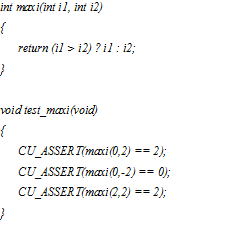
\includegraphics[scale=1]
{fig4}


CUnit provides a set of assertions for testing logical conditions.  The success or failure of these assertions is tracked by the framework, and can be viewed when a test run is complete. Each assertion tests a single logical condition, and fails if the condition evaluates to FALSE. Upon failure, the test function continues unless the user chooses the `xxx\_FATAL'  version of an assertion. In that case, the test function is aborted and returns immediately.  \\

However all of the unit test tools for C are available for user space application programs. There are some kernel specific limitations which prevent development of a generic unit testing framework for Linux kernel modules.  Few of the complexities of testing a kernel code (a device driver functions or a kernel module functions)  using a standard unit test tools like Cunit or CuTest are listed below.\\
\begin{itemize}
\item Unit testing kernel level code using the standard tool is highly impossible. Either the tool has to be ported into a kernel module so that it can access the kernel code at unit level or the kernel code has to be moved to user space, but moving the kernel code to user space is not possible due to the strong dependency between the kernel APIs. For example the memory allocation is done in kernel code using the function kmalloc() but whereas the same is done at user space using malloc().\\

\item Unit testing from user space using general applications doesn’t solve the purpose.  For example, if a function in a kernel module needs to be verified, then a particular application level call which executes the particular kernel modules function after passing through many kernel layers need to be identified and executed. But this doesn’t solve the primary purpose of unit testing. A new method is required to directly invoke the kernel function with proper prerequisites setup so the kernel function alone can be executed with varying arguments to the same. 
\item  Even if the unit test tools like C-Unit or CUTest are ported to kernel space, the test cases cannot be executed directly from a kernel module as the execution of test code requires either a user level process context or a specific kernel thread.  Developing either of them for individual modules is costly and will consume majority of testing resources.
\item  The kernel modules have high level of interactions with them so applying a generic method without knowing the internal communication between kernel modules may not yield a proper test tool.

\end{itemize}


